\section{流输入/输出\texttt{iostream}}
本节所介绍的内容不仅适用于标准流输入/输出,也适用于字符串输入/输出和文件输入/输出。毕竟,它们对应的类都直接或间接地继承自 \lstinline@std::basic_istream@ 或 \lstinline@std::basic_ostream@,所以也有这些类的功能。\par
\subsection*{输入信息中的分隔符}
有的时候我们会遇到需要一次性输入多个数据的情况,这时我们的选择是用空格来分隔开。
\begin{lstlisting}
    std::istringstream sin {"25 1.3 Alan Turing"}; //需要包含sstream库
    std::cin.rdbuf(sin.rdbuf()); //重定向之后,cin的源就是sin中存的字符串
    int i;
    double d;
    char str[50];
    std::cin >> i >> d >> str;
    std::cout << i << '\n' << d << '\n' << str << '\n';
    std::cin >> str;
    std::cout << str << std::endl;
\end{lstlisting}
在这里我们使用了 \lstinline@std::istringstream@ 对象来存储一段字符串输入,然后让 \lstinline@std::cin@ 重定向到它。这样,我们就可以省去了运行程序时再输入内容的麻烦,而是直接把输入内容也写到代码里——无论输入流的源是什么,它们的效果都相同。\par
这段代码的运行结果是:\\\noindent\rule{\linewidth}{.2pt}\texttt{
25\\
1.3\\
Alan\\
Turing
}\\\noindent\rule{\linewidth}{.2pt}\par
在输入信息中,\texttt{25} 和 \texttt{1.3} 之间的空格就是一个\textbf{分隔符(Delimiter)}。 在处理输入的时候,程序一旦遇到这样的分隔符,就会暂停读取输入,并把当前已经获得的输入内容(字符 \texttt{2} 和 \texttt{5} )处理成一个数据,赋值给 \lstinline@i@;接下来,它会无视下一位的空格\footnote{这个空格符作为流的一部分,仍然要被程序所接收。但是当 \lstinline@std::cin@ 发现这是一个空格符的时候,它就会什么也不做——表现出来就是无视了空格。},把后面的 \texttt{1.3} 读入其中,然后再次在空格符之前止步,把这些字符处理成数据,赋值给 \lstinline@d@;接收,它又在另一个空格符之前停下,把 \texttt{Alan} 复制给 \lstinline@str@;最后,它在文件结尾字符 \texttt{EOF}\footnote{EOF(End of file)不是一个ASCII字符(虽然它有未指明的ASCII值,通常为\texttt{-1}),但它可以用来表示文件的结尾。当输入流对象读到文件结尾字符时,输入流对象的状态发生改变,输入也就停止了。}之前停下,把 \texttt{Turing} 复制给 \lstinline@str@。于是我们就能看到这样的输出结果了。(图13.3)\par
\begin{figure}[htbp]
    \centering
    
\includegraphics[width=.4\textwidth]{../images/generalized_parts/13_input_with_space_delimiter.drawio.png}
    \caption{含空白分隔符的输入信息处理}
    \footnotesize{颜色用以区分不同批次的输入,下同} 
\end{figure}
在C++中,不止空格(ASCII:32)可以作为分隔符,制表符和换行符等(ASCII:9-13)也都可以作为分隔符。所以我们用空格也行,用换行也行,都能作分隔符——不过,在键盘输入的情况下,换行符还可以作为``确认输入''的按键,我们待会再讲。\par
读者还可以试试这段代码:
\begin{lstlisting}
    std::istringstream sin {"12.34.56."};
    std::cin.rdbuf(sin.rdbuf()); //重定向之后,cin的源就是sin中存的字符串
    int i;
    double d;
    char str[50];
    std::cin >> i >> d >> str;
    std::cout << i << '\n' << d << '\n' << str << '\n';
\end{lstlisting}
这段代码的输出是\\\noindent\rule{\linewidth}{.2pt}\texttt{
12\\
0.34\\
.56.
}\\\noindent\rule{\linewidth}{.2pt}\par
这里没有空格分隔符,那么输入流对象是怎么对输入信息进行划分的呢?答案是:如果出现了非预期的字符,那么就地止步。\par
比如说,在输入 \lstinline@int@ 型数据的时候,预期之内的字符只能有数一堆字(如果以十六进制输入,那还会有部分大小写字母)和最多一个负号。那么其它的字符,无论是空格符,还是小数点,还是其它的字母,它们全都不应该输入到整型数据当中。所以程序读到小数点字符的时候,就会暂停读入,把已经读入的部分 \texttt{12} 处理成数据,赋值给 \lstinline@i@;\par
接下来输入的 \lstinline@double@ 型数据允许有至多一个小数点。所以它可以正常地读取 \texttt{.34} ——接下来遇到又一个小数点的时候,它就该暂停了,因为一个小数不可能有两个小数点;\par
最后,对于 \lstinline@char[50]@ 来说,它就可以读取任意的ASCII字符了,于是后面的内容都会被 \lstinline@str@ 截获。(图13.4)当然,这里的输入还是会受到分隔符的影响,我们待会儿再谈。\par
\begin{figure}[htbp]
    \centering
    
\includegraphics[width=.4\textwidth]{../images/generalized_parts/13_input_without_delimiter.drawio.png}
    \caption{非预期输入的处理}
\end{figure}
读者还记得我们在第三章中设计过的简易计算器吗?以下是其中的输入部分代码:
\begin{lstlisting}
    double num1, num2, result; //定义两个操作数num及结果值result
    char op; //定义一个字符用来存储运算符输入
    cin >> num1 >> op >> num2; //依次输入左操作数、运算符和右操作数
\end{lstlisting}
我们现在可以随便编一个合理输入,比如说 \texttt{1+.2},这个程序完全能理解我们想表达 \texttt{1.0 + 0.2} 的意思。这是因为,\texttt{+} 对于 \lstinline@double@ 型的输入来说是非预期的输入,所以 \lstinline@num1@ 的输入会停留在 \texttt{1} 这里。对于 \lstinline@char@ 型的输入来说,它只能读取下一个(非空白)字符,所以 \texttt{+} 就赋值给它了;接下来的 \texttt{.2} 当然就归 \lstinline@num2@ 了。(图13.5)\par
\begin{figure}[htbp]
    \centering
    
\includegraphics[width=.4\textwidth]{../images/generalized_parts/13_input_for_calculator.drawio.png}
    \caption{计算器程序中的输入处理}
\end{figure}
\subsection*{\texttt{getline}与\texttt{get}成员函数}
以空格为隔符的输入处理,当然极大地方便了我们输入一般的数值数据。但是在输入字符串的时候,可能就未必这么方便了。我们在第五章就介绍过,在字符串的输入过程中,如果我们想要输入的字符串(比如英文名)本身就带有空白字符,那么 \lstinline@std::istream::operator>>@ 会在空白字符处断开,把我们的输入理解成两个字符串。\par
为了解决这个问题,我们就要使用 \lstinline@getline@ 或 \lstinline@get@ 成员函数了。对于这两个成员函数来说,我们都可以自定义分隔符,让它们读取分隔符以外的ASCII字符。当遇到分隔符时,它们会停下来(其中,\lstinline@getline@ 会把分隔符也一并提取,而 \lstinline@get@ 不会)。以下是示例:
\begin{lstlisting}
    std::istringstream sin {"Alan Turing\nClaude Shannon\nBjarne Stroustrup"};
    //输入内容预先存于sin中
    std::cin.rdbuf(sin.rdbuf()); //重定向之后,cin的源就是sin中存的字符串
    char name[3][40] {}; //定义3个40长度char数组
    for (int i = 0; i < 3; ++i)
        std::cin.getline(name[i], 40); //向name[i]中最多输入40字符,结束符为'\n'
    for (auto str : name)
        std::cout << str << std::endl;
\end{lstlisting}
读者也可以不做这个重定向,而是直接用键盘输入,其中的 \lstinline@'\n'@ 按Enter键表示就好。这段代码的运行结果如下:\\\noindent\rule{\linewidth}{.2pt}\texttt{
Alan Turing\\
Claude Shannon\\
Bjarne Stroustrup
}\\\noindent\rule{\linewidth}{.2pt}\par
对于 \lstinline@getline@ 成员函数来说,如果我们不提供分隔符参数,那么它将以换行符为分隔符\footnote{但是,它与提供分隔符的另一同名函数之间是重载关系,而不是有默认参数关系。};其它的空白字符都将被当作是输入的一部分。所以我们就能看到输出结果中的这个样子。除此之外,\lstinline@getline@ 也将把分隔符一并提取,但并不将其视为字符串的一部分。\par
我们可以自行提供分隔符参数。在这种情况下,分隔符就不是 \lstinline@'\n'@ 而是我们提供的那个字符了。
\begin{lstlisting}
    std::istringstream sin {"ab-cd-e-fgh"};
    std::cin.rdbuf(sin.rdbuf()); //重定向之后,cin的源就是sin中存的字符串
    char name[5][10] {}; //定义5个10长度char数组
    for (int i = 0; i < 5; ++i)
        std::cin.getline(name[i], 10, '-');
        //向name[i]中最多输入10字符,结束符为'-'
    for (auto str : name)
        std::cout << str << std::endl;
\end{lstlisting}\newpage
这段代码的运行结果是\footnote{输出结果应该有六行。我将末尾的换行符省略,这样还剩下五行,其中第五行是空串的输出,所以看上去没有任何内容。}:\\\noindent\rule{\linewidth}{.2pt}\texttt{
ab\\
cd\\
e\\
fgh\\
\newline
}\\\noindent\rule{\linewidth}{.2pt}
不难看出,\lstinline@getline@ 成员函数把输入内容从 \lstinline@'-'@ 字符处拆开,然后把拆分出来的输入信息存入每个 \lstinline@name[i]@ 中,并在末尾都加上了字符串结束符 \lstinline@'\0'@(这是很重要的)。而分隔符本身并没有塞到字符串中,它被忽略了。\par
\lstinline@get@ 成员函数的重载版本比 \lstinline@getline@ 要多,而其中也包含有带分隔符的重载。但是 \lstinline@get@ 函数与 \lstinline@getline@ 不同的地方就在于,\lstinline@get@ 函数不会吞掉分隔符,它会把分隔符继续保留在输入流当中,这个分隔符可以被下次的输入所提取。
\begin{lstlisting}
    //其它代码同上,省略
    for (int i = 0; i < 5; ++i)
        std::cin.get(name[i], 10, '-');
        //用get成员函数向name[i]中最多输入10字符,结束符为'-'(能奏效吗)
\end{lstlisting}
分隔符处理方面的细微差别能带来巨大的影响,我们一看输出结果便知\footnote{这里有五行输出,其中后四行都是空串输出。}:\\\noindent\rule{\linewidth}{.2pt}\texttt{
ab\\
\newline
\newline
\newline
\newline
}\\\noindent\rule{\linewidth}{.2pt}
这就是 \lstinline@get@ 函数没有吞掉分隔符导致的问题。我们想,如果 \lstinline@'-'@ 还在输入流当中的话,那么下一次 \lstinline@get@ 函数调用的时候,读到的第一个字符不就是分隔符了吗?在这种情况下,\lstinline@get@ 函数就没有读到任何的内容(失败),那么 \lstinline@name[1]@ 当然就变成空串了,\lstinline@name[2]@ 及其之后的当然也都变成空串了。(图\par
\begin{figure}[htbp]
    \centering
    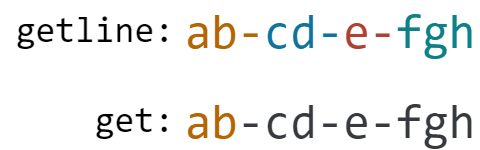
\includegraphics[width=.4\textwidth]{../images/generalized_parts/13_getline_vs_get.drawio.png}
    \caption{\lstinline@getline@ 与 \lstinline@get@ 成员函数处理分隔符的差别}
\end{figure}
所以说到底是用 \lstinline@getline@ 还是 \lstinline@get@,我们需要根据具体的情况和我们的需求加以选择。如果我们希望分隔符留在输入流中听候发落,那就用 \lstinline@get@;如果我们不希望分隔符还留在输入流中继续产生影响,那就用 \lstinline@getline@。\par
\lstinline@get@ 成员函数还有其它的重载,比如说这两个:
\begin{lstlisting}
int_type basic_istream::get(); //(1)
basic_istream& basic_istream::get(char_type& ch); //(2)
\end{lstlisting}\par
它们的作用其实是一样的,都是读取输入流中的下一个字符。对于(1)来说,它的返回值就是读取到的字符的ASCII值——是一种整型数据;而对于(2)来说,它会把读取到的字符赋值给 \lstinline@ch@ 参数,而返回值正是调用这个函数的对象。\par
它们各有用途。就以 \lstinline@get()@ 来说吧,我们可以用它来``清空本行输入流''。具体方法倒也很简单:
\begin{lstlisting}
    while (std::cin.get() != '\n')
        continue; //或者直接空语句
\end{lstlisting}
这个操作的意思就是:持续地从输入流中一个个字符地读取,并与 \lstinline@'\n'@ 比较,直到条件不满足,也就是读入的字符与 \lstinline@'\n'@ 相等。就这么简单。\par
你还记得我们曾在第一章开篇就讲过,如果你的IDE在程序结束时产刻关闭窗口导致我们来不及看程序运行结果,那么我们可以在主函数的 \lstinline@return 0@ 之前加上一个 \lstinline@cin.get()@。其实这就是为了等待键盘输入——我们必须人为地再进行一次输入(无论是按Enter还是按了别的再按Enter),这样程序才会真正意义上结束。\par
但是有的时候,我们用一个 \lstinline@cin.get()@ 还不够。
\begin{lstlisting}
    int i;
    std::cin >> i; //这次不重定向了,用键盘输入
    std::cout << std::cin.get(); //先读取下一个输入流字符,再输出其ASCII值
\end{lstlisting}
这个程序的运行结果是这样的(粗体表示用户输入内容):\\\noindent\rule{\linewidth}{.2pt}\texttt{
\textbf{5}\\
10
}\\\noindent\rule{\linewidth}{.2pt}\\
当我们输入\textbf{5}并按下Enter键的时候,程序并没有等我们再按一次Enter,而是输出 \lstinline@std::cin.get()@ 的结果并结束运行了,这是为什么呢?\par
其实答案就在我们按下的那次Enter键当中。当我们按下Enter时,我们实际上进行了两项操作:确认我们的输入内容(把这一整行的输入添加到输入流中),并向输入流中添加一个换行符。\par
而 \lstinline@std::istream::operator>>@ 在读取内容时,不会把分隔符(也就是空白字符)一并解析,而是留在输入流中。于是当程序完成 \lstinline@std::cin>>i@ 之后,输入流中还剩下一个 \lstinline@'\n'@ 没有读呢!这个换行符当然就被后面的 \lstinline@std::cin.get()@ 读到,这也就是为什么程序没等我们再按Enter就输出,而且输出内容还是 \lstinline@10@(换行符的ASCII值为10)。\par
解决这个问题的方法也很简单:用两个 \lstinline@cin.get()@ 就好了。这样一来,输入流中遗留的 \lstinline@'\n'@(如果有的话)会被第一个 \lstinline@get()@ 提取,而接下来我们必须要人为地用键盘再进行一次输入了。\par
至于 \lstinline@std::string@ 类的相关整行输入操作,我们可以用 \lstinline@string@ 库中定义的 \lstinline@std::getline@ 函数来完成。它的声明如下:
\begin{lstlisting}
template<class CharT, class Traits, class Allocator>
std::basic_istream<CharT, Traits>& getline(
    std::basic_istream<CharT, Traits>& input,
    std::basic_string<CharT, Traits, Allocator>& str,
    CharT delim
);
template<class CharT, class Traits, class Allocator>
std::basic_istream<CharT, Traits>& getline(
    std::basic_istream<CharT, Traits>& input,
    std::basic_string<CharT, Traits, Allocator>& str
); //将以'\n'为分隔符
\end{lstlisting}\par
套路差不多,只不过它是非成员函数,我们需要写成 \lstinline@std::getline(std::cin,str)@ 这样来调用它而已。\par
\subsection*{流对象的状态}
我们说,在输入过程中,若是遇到了非预期的字符,程序就会止步于此,把已经读到的字符赋值给相应的实参。但是你有没有想过,如果一上来就让它读一个非预期的字符,那会发生什么?
\begin{lstlisting}
    std::istringstream sin {".123\n"};
    std::cin.rdbuf(sin.rdbuf());
    int i;
    std::cin >> i;
\end{lstlisting}
在这里,既然 \lstinline@i@ 是个整型数据,那么小数点字符就是非预期的输入。但是这个时候输入流对象还没有读任何内容,那么问题也就随之发生。\par
对于上面的 \lstinline@std::cin.get(name[i],/*...*/)@ 来说也有这个问题。我们可以想一想,当它打算输入 \lstinline@name[1]@ 却发现第一个字符就是分隔符的时候,它也同样什么都没读到。\par
这些``什么都没读到''的情形通常意味着用户提供了不合理的输入,这是危险的。在这种情况下,这个输入流对象(比如 \lstinline@std::cin@)会进入``读取失败''状态。在这种状态下,这个对象不再正常进行输入工作,所有与它相关的输入操作,无论 \lstinline@>>@ 还是 \lstinline@getline@,都会不予执行直接跳过。\par
除了``读取失败''状态以外,还有另外两种状态:文件结尾和错误。它们都定义在 \lstinline@std::ios_base@ 中,无论输入类还是输出类都有这些状态属性——不过我们一般只用来研究输入,因为输入中有太多不可预测行为,而输出中很少出现这些问题。\par
要想获取这些状态变量的值,我们可以用成员函数 \lstinline@fail()@, \lstinline@eof()@ 和 \lstinline@bad()@。它们的返回值都是 \lstinline@bool@ 类型的,如果值为 \lstinline@true@,就说明这个对象存在该异常状态;如果返回值为 \lstinline@bool@,就说明这个对象不存在该异常状态。还有一个成员函数 \lstinline@good()@,仅当该对象没有任何异常状态时才返回 \lstinline@true@,否则返回 \lstinline@false()@。\par
现在我们可以回去看一下那个用了 \lstinline@std::cin.get(name[i],/*...*/)@ 的代码到底发生了什么。
\begin{lstlisting}
    std::istringstream sin {"ab-cd-e-fgh"};
    std::cin.rdbuf(sin.rdbuf()); //重定向之后,cin的源就是sin中存的字符串
    char name[5][10] {}; //定义5个10长度char数组
    for (int i = 0; i < 5; ++i) {
        std::cin.get(name[i], 10, '-');
        std::cout << std::cin.fail() << ' '; // 0 1 1 1 1
    }
\end{lstlisting}
我已经把这段代码的运行结果标记在注释中了。读者可以看到,在第二次使用 \lstinline@get@ 之后 \lstinline@fail()@ 状态就已经变成了 \lstinline@true@,这也就是说,其后的那些 \lstinline@std::cin.get(/*...*/)@ 其实都什么也没做。\par
此外,你可别以为用了 \lstinline@getline@ 的版本看上去好像一切正常,我们就可以高枕无忧了。如果你在这个循环中检测一下输入状态,也会发现存在问题。\pagebreak
\begin{lstlisting}
    std::istringstream sin {"ab-cd-e-fgh"};
    std::cin.rdbuf(sin.rdbuf()); //重定向之后,cin的源就是sin中存的字符串
    char name[5][10]; //定义5个10长度char数组
    for (int i = 0; i < 5; ++i) {
        std::cin.getline(name[i], 10, '-');
        std::cout << std::cin.fail() << ' '; // 0 0 0 0 1
    }
\end{lstlisting}
其实我们分析一下马上就能想明白,毕竟 \lstinline@sin@ 中提供的内容只够输入四个字符串。那么对于第五个字符串来说,\lstinline@std::cin@ 已经读不到新的内容了。这种情况下,\lstinline@std::cin@ 也会被置为失败状态(其实还有个文件结尾状态)。这个状态会像狗皮膏药一样一直贴在它身上,往后只要我们用 \lstinline@std::cin@ 来进行输入,它就会什么也不做,罢工。\par
我们可以用 \lstinline@clear@ 成员函数来清除错误状态。
\begin{lstlisting}
void basic_ios::clear(
    std::ios_base::iostate state = std::ios_base::goodbit
);
\end{lstlisting}
我们可以自定义状态并设置我们想要的值;但是泛讲篇中我们就不关注那么多细节了,直接用默认值形式就好。\par
但是你别忘了,引发 \lstinline@fail()@ 状态的那些输入字符还在输入流里呢。如果我们只是清除了错误状态,但没有清理那些引发错误内容,那就治标不治本。等下我们要用 \lstinline@std::cin@ 来输入的时候它又要出错了。所以我们需要两步操作:
\begin{lstlisting}
void input_clear(std::istream &in = {std::cin}) {
    in.clear(); //先用clear清除错误状态,要不然等下也没法用它来get
    while (in.get() != '\n') { } //清除本行输入
}
\end{lstlisting}
这样,一个稳妥的状态恢复/问题消除流程就完成了。这也就是我们从第三章开始就在用的那个\linebreak\lstinline@input_clear@ 函数。\par
更多相关方面的操作,我们就留到精讲篇再谈。\par
\subsection*{格式化输出}
看完了输入,我们再来看看输出。\lstinline@std::ostream@ 类提供了一些默认的输出格式,比如说 \lstinline@bool@ 数据都以整数形式输出,较大或较小的浮点数以科学记数法形式输出。\par
但是在实际操作过程中,甲方难免会给你提出一些奇奇怪怪的输出格式需求,比如说——
\begin{itemize}
    \item ``你把这个小数……这个小数,都保留三位小数啊。''
    \item ``你把这几个数据对齐啊。要右对齐的。''
    \item ``你输出十六进制数的时候能不能大写?''
\end{itemize}
所幸,对于一些基本的格式需求来说,\lstinline@std::ios_base@ 中已经定义了一系列的格式化函数和格式化标记。像上面提到的这些需求,在C++中可以通过调用相关的函数来实现,不需要麻烦我们自己写一大堆代码了。\par
\subsubsection*{布尔数据输出}
我们可以用 \lstinline@setf@ 成员函数和一系列格式标记常量来改变输出的格式,或者用 \lstinline@unsetf@ 成员函数进行逆操作。\par
我们先来看一个比较简单的例子,那就是布尔型变量的输出。C++默认以整数值的形式输出 \lstinline@bool@ 数据,我们可以改变格式标记,让它能够输出 \lstinline@true@/\lstinline@false@ 来。\par
\lstinline@std::ios_base::boolalpha@ 是一个常量,它有自己的含义。我们不必去细究它的值是什么——它的值只是一种编码而已。
\begin{lstlisting}
    std::cout.setf(std::ios_base::boolalpha); //设置boolalpha格式标记
    std::cout << true << ' ' << false << std::endl;
    std::cout.unsetf(std::ios_base::boolalpha); //撤销boolalpha格式标记
    std::cout << true << ' ' << false << std::endl;
\end{lstlisting}
这段代码的运行结果是:\\\noindent\rule{\linewidth}{.2pt}\texttt{
true false\\
1 0
}\\\noindent\rule{\linewidth}{.2pt}\\
很简单,不用我多说了吧。\par
\subsection*{定点/浮点表示}
表示一个浮点数有两种基本格式。一种是不带指数的定点表示,把各个位数都输出出来:对于整数部分,有多少位就输出多少位;对于小数部分,按规定的精度来输出,我们稍后讲精度问题。另一种是浮点表示,也就是把所有数据都用科学记数法表示,而精度也按规定值执行。\par
C++的默认输出格式并不是这两种基本格式之一,它是一种最方便我们阅读的格式。如果这个数很大或者很小,这时才会使用科学记数法;如果这个值不很大,但几乎就是整数(小数部分即便显示出来也约等于零),那它就会像整数一样输出;如果这个值是小数,那它就会根据小数位数来输出。但我们总会有特殊的需要,所以我们可以修改表示方法,在``默认''``定点''``浮点''三者之间切换。这时我们也可以使用 \lstinline@setf@ 和 \lstinline@unsetf@ 来进行格式转换。
\begin{lstlisting}
    std::cout << 1e10 << ' ' << 12e-7 << std::endl; //默认格式输出
    std::cout.setf(std::ios_base::fixed, std::ios_base::floatfield);
    //设为定点格式输出,需要使用掩码std::ios_base::floatfield
    std::cout << 1e10 << ' ' << 12e-7 << std::endl;
    std::cout.setf(std::ios_base::scientific, std::ios_base::floatfield);
    //设为浮点格式输出,需要使用掩码std::ios_base::floatfield
    std::cout << 1e10 << ' ' << 12e-7 << std::endl;
    std::cout.unsetf(std::ios_base::floatfield);
    //改回默认格式,同样需要使用掩码std::ios_base::floatfield
    std::cout << 1e10 << ' ' << 12e-7 << std::endl;
\end{lstlisting}\newpage
这段代码的输出结果是:\\\noindent\rule{\linewidth}{.2pt}\texttt{
1e+10 1.2e-06\\
10000000000.000000 0.000001\\
1.000000e+10 1.200000e-06\\
1e+10 1.2e-06
}\\\noindent\rule{\linewidth}{.2pt}\par
代码应该不需要我多讲了,我只介绍一下\textbf{掩码(Mask)}。对于 \lstinline@std::ios_base@ 对象来说,它们的那些格式化标记并不是分别存储在好多个布尔变量中的,而是存到了同一个数据中\footnote{前文也提及,一个 \lstinline@bool@ 数据只需表示两个值,但却要占据一个字节8比特的内存空间,这就浪费了7个比特,太不经济。}。但是如果它们存在了同一个数据中,我们怎么能保证修改一个标记的同时保证其它的标记不受影响呢?掩码就可以帮助我们屏蔽掉一个数据中不需要的部分,我们只能操作一定范围内的信息。掩码的原理要通过位运算来讲解,而在泛讲篇中我们就不谈了。\par
\subsubsection*{进制与进制前缀}
C++标准库对于进制转换的支持比较简陋。不过我们可以很容易地以十进制(默认)、八进制或十六进制来进行输入/输出。\par
在变换输入/输出进制的时候,我们也可以使用 \lstinline@setf@ 成员函数。八进制使用 \lstinline@std::ios_base::oct@;十进制使用 \lstinline@std::ios_base::dec@\footnote{实际上也可以直接 \lstinline@unsetf(std::ios_base::basefield)@。};十六进制使有 \lstinline@std::ios_base::hex@。关于这个进制的掩码是 \lstinline@std::ios_base::basefield@。
\begin{lstlisting}
    std::cout.setf(std::ios_base::oct, std::ios_base::basefield); //设为八进制
    std::cout << 59 << std::endl; //73
    std::cout.setf(std::ios_base::hex, std::ios_base::basefield); //设为十六进制
    std::cout << 59 << std::endl; //3b
    std::cout.setf(std::ios_base::dec, std::ios_base::basefield); //设为十进制
    std::cout << 59 << std::endl; //59
\end{lstlisting}\par
十六进制输入的时候,默认是用小写字母的;如果你想要让它用大写字母,那也很简单,用 \lstinline@std::ios_base::uppercase@ 就好。这会让十六进制输出采用大写字母;也会让浮点表示中的 \lstinline@e@ 采用大写字母。
\begin{lstlisting}
    std::cout.setf(std::ios_base::uppercase); //某些输出采用大写
    std::cout.unsetf(std::ios_base::uppercase); //如果你想要恢复
\end{lstlisting}\par
为了区分不同进制的整数,在C++中我们可以为八进制数加上 \lstinline@0@ 前缀,为十六进制数加上 \lstinline@0x@ 前缀来区分,比如 \lstinline@031@ 就是十进制的 \lstinline@25@,而 \lstinline@0x31@ 就是十进制的 \lstinline@49@。而在输出的时候我们好像没有体现出这点来。我们可以用 \lstinline@std::ios_base::showbase@ 来输出带前缀的格式,从而区分不同进制。
\begin{lstlisting}
    std::cout.setf(std::ios_base::showbase); //显示前缀对应的进制底数
    std::cout << 31 << std::endl; //31
    std::cout.setf(std::ios_base::oct, std::ios_base::basefield); //设为八进制
    std::cout << 031 << std::endl; //031
    std::cout.setf(std::ios_base::hex, std::ios_base::basefield); //设为十六进制
    std::cout << 0x31 << std::endl; //0x31
    std::cout.unsetf(std::ios_base::showbase); //取消显示前缀对应的进制底数
\end{lstlisting}\par
\subsubsection*{浮点精度设置}
\lstinline@std::cout@ 的默认浮点精度是6,也就是说在以定点/浮点格式表示时,它将输出到小数点后的6位。我们可能需要自行更改这个精度值,以符合我们的输出要求。这时就要用到成员函数 \lstinline@precision@ 了。
\begin{lstlisting}
streamsize ios_base::precision()const; //(1)	
streamsize ios_base::precision(streamsize new_precision); //(2)
\end{lstlisting}
其中(1)只负责返回值,而(2)可以修改精度要求。它们的返回值都是修改之前的精度值。\par
有了这个成员函数之后,我们就可以让定点和浮点形式的输出结果限制到指定的小数位;至于默认输出格式,那是不受影响的。这方面的例子就请读者自行尝试吧。\par
\subsubsection*{设置宽度与对齐方式}
我们可以用 \lstinline@iomanip@ 库中的 \lstinline@std::setw@ 函数来设置输出内容的宽度。设置宽度的意思是,为这段内容单独定制一个输出宽度,如果输出内容实际上没有那么宽,那程序也会拿填充符(比如空格)填上,总之不会让下一个输出内容占据它。这种操作在我们想要一行行按表格形式输出时会非常有用,以下是一个示例:
\lstinputlisting[caption=\texttt{output\_info.cpp}]{../code_in_book/13.1/output_info.cpp}
这段代码的运行结果如下:\\\noindent\rule{\linewidth}{.2pt}
\begin{verbatim*}
     Name  Sex  Age  Height
    Alice    F   28    165.1
      Bob    M   32   185.45
  Charlie    M   45    175.3
    Diana    F   37   170.26
\end{verbatim*}\noindent\rule{\linewidth}{.2pt}\\
读者会发现,在这里它们都是右对齐的——这也是默认的对齐状态。\par
另外,\lstinline@Height@ 看起来没有与下面的数据对齐,这是怎么回事呢?其实原因在于,我们紧随 \lstinline@std::setw(9)@ 之后输出的内容是 \lstinline@"Height\n"@。这里的 \lstinline@'\n'@ 虽然体现出来是换行,但是它也被当作内容长度的一部分。\par
注意,\lstinline@setw@ 只对下一次的输出有作用,而对之后的输出不再起作用。比如说\linebreak\lstinline@std::cout<<std::setw(2)<<1<<2<<3@,输出的结果将是\texttt{ 123}而不是\texttt{ 1 2 3}。\par
我们可以更改 \lstinline@setw@ 作用下的内容对齐方式:\lstinline@std::ios_base::right@ 是默认的右对齐,\linebreak\lstinline@std::ios_base::left@ 是左对齐,\lstinline@std::ios_base::internal@ 是两端对齐\footnote{怎么理解这个 \lstinline@internal@ 呢?我们可以理解成,在符号(比如负号,美元符号或者 \lstinline@0@, \lstinline@0x@ 前缀)和数字部分之间添加填充符,把左右的内容顶到这个宽度区域的两侧。}。它们的掩码是\linebreak\lstinline@std::adjustfield@。
\begin{lstlisting}
    std::cout.setf(std::ios_base::hex, std::ios_base::basefield); //十六进制输出
    std::cout.setf(std::ios_base::showbase); //显示前缀
    std::cout << std::setw(8) << 123 << '\n'; //默认右对齐
    std::cout.setf(std::ios_base::left, std::ios_base::adjustfield);
    std::cout << std::setw(8) << 123 << '\n';
    std::cout.setf(std::ios_base::internal, std::ios_base::adjustfield);
    std::cout << std::setw(8) << 123 << '\n';
\end{lstlisting}
这段代码的运行结果是:\\\noindent\rule{\linewidth}{.2pt}
\begin{verbatim*}
    0x7b
0x7b    
0x    7b
\end{verbatim*}\noindent\rule{\linewidth}{.2pt}
\subsection*{输入/输出操纵符}
前面提到过的那些格式设定虽然有用,但是写起来还是太麻烦了,有些还需要用掩码,挺费事的。而 \lstinline@ios@, \lstinline@istream@, \lstinline@ostream@\footnote{前三个库其实已经包含在 \lstinline@iostream@ 中了,我们可以省去写它们的麻烦。}, \lstinline@iomanip@ 等库中定义的输入输出操纵符能够大大简化这些操作。\par
举例来说,如果我们想要输出左对齐,只需要使用 \lstinline@ios@ 库中的 \lstinline@std::left@ 作为 \lstinline@<<@ 的右参数就行,像这样:
\begin{lstlisting}
    std::cout << std::left; //等效于下面这句
    //std::cout.setf(std::ios_base::left, std::ios_base::adjustfield);
\end{lstlisting}
这就方便多了嘛。\par
至于有些不是靠掩码而是靠 \lstinline@unsetf@ 成员函数来实现的格式控制,C++库中也有对应的输入/输出操纵符,一般是这样的:
\begin{lstlisting}
    std::cout << std::boolalpha; //布尔值用true/false输出
    std::cout << std::noboolalpha; //回到默认状态,用1/0输出
    std::cout << std::showbase; //显示进制前缀
    std::cout << std::noshowbase; //回到默认状态,不显示进制前缀
\end{lstlisting}\par
这些输入/输出操纵符的作用期限是整个运行期;只要不改,它就一直保持这种输入格式;而不像 \lstinline@std::setw@ 这样仅限一次输出有效。\par
其它输入输出操纵符的道理基本相同,我就不再赘述,详见\href{https://zh.cppreference.com/w/cpp/io/manip}{输入/输出操纵符 - cppreference.com}。\par
